
\section{Two certified interior critical-line crossings}

\noindent
The unchanged family is
\[
 F(s,t)=\zeta(s,1+t),\qquad t>-1.
\]
This note proves that there are two isolated pairs with \(0<t<1\),
\(s=\tfrac12+i\gamma\), and \(F(s,t)=0\). Each zero is simple in
\(s\), and its local zero curve crosses the critical line with a certified
nonzero real velocity. These are rigorous local results obtained by ball
arithmetic and a contraction proof. The two seeds were suggested by
numerical continuation; the proofs do not identify either zero with an
initially indexed Riemann zero, and do not certify an entire continued
path. They give no assertion about all zeros of any one member of the
family or a proof of the Riemann hypothesis.

\subsection{Analytic family and the exact real Jacobian}

\begin{hxctheorem}\label{hxc:analytic}
Put \(a=1+t\). The function \(F\) is jointly holomorphic for
\(\Re s>-1\), \(s\ne1\), \(\Re a>0\), with the logarithm chosen on
the right half-plane. It agrees with \(\sum_{n=0}^\infty(n+a)^{-s}\)
when \(\Re s>1\). At the points used below,
\begin{equation}\label{hxc:flow}
 F_t(s,t)=-s\zeta(s+1,1+t).
\end{equation}
Define the real map, in the specified coordinate order,
\[
 G:\R\times(-1,\infty)\longrightarrow\R^2,
 \qquad
 G(\gamma,t)=
 \begin{pmatrix}\Re F(\tfrac12+i\gamma,t)\\
                 \Im F(\tfrac12+i\gamma,t)\end{pmatrix}.
\]
Its Jacobian is exactly
\begin{equation}\label{hxc:jacobian}
 DG(\gamma,t)=
 \begin{pmatrix}
 -\Im F_s&\Re F_t\\
 \Re F_s&\Im F_t
 \end{pmatrix}_{(s,t)=(1/2+i\gamma,t)}.
\end{equation}
\end{hxctheorem}

\begin{proof}
For completeness, write \(\widetilde B_2(x)=u^2-u+1/6\), where
\(u=x-\lfloor x\rfloor\). Two integrations by parts on each interval
\([n,n+1]\), followed by summation, give, for
\(f(x)=(x+a)^{-s}\),
\[
 \sum_{n=0}^{N-1}f(n)
 =\int_0^N f(x)\dd x+\frac{f(0)-f(N)}2
  +\frac{f'(N)-f'(0)}{12}
  -\frac12\int_0^N\widetilde B_2(x)f''(x)\dd x.
\]
The endpoint values used here are \(B_2(0)=B_2(1)=1/6\) and
\(B_2'(0)=-1\), \(B_2'(1)=1\); they give every displayed sign.
Taking \(N\to\infty\) first for \(\Re s>1\) yields
\begin{equation}\label{hxc:continuation}
 \zeta(s,a)=\frac{a^{1-s}}{s-1}+\frac{a^{-s}}2
  +\frac{s}{12}a^{-s-1}
  -\frac{s(s+1)}2\int_0^\infty
       \widetilde B_2(x)(x+a)^{-s-2}\dd x.
\end{equation}
On compact subsets of the claimed domain, \(\widetilde B_2\) is bounded,
the tail has size at most a fixed constant times \(x^{-\Re s-2}\),
and derivatives add only logarithmic factors or further negative powers
of \(x+a\). Consequently the integral and its local parameter
derivatives converge uniformly when \(\Re s>-1\). This proves the
claimed continuation and joint holomorphy. Termwise differentiation of
the original absolutely convergent series for \(\Re s>1\) gives
\eqref{hxc:flow}. Analytic continuation gives the same identity in a
neighborhood of every box below. Finally \(\partial_\gamma F=iF_s\);
taking its real and imaginary parts proves \eqref{hxc:jacobian}.
\end{proof}

\subsection{Exact input boxes and a completed contraction certificate}

Every terminating decimal in this section denotes the exact rational
number specified by its digits. Set \(r=10^{-12}\), and use the centers
\begin{align*}
 c_{A,\gamma}&=41.83377298972885114660494764956585698672,\\
 c_{A,t}&=0.95095300424959108490589251950106981050,\\
 c_{B,\gamma}&=47.04386821148998246126561185165482331798,\\
 c_{B,t}&=0.85870425944212436115567453829890140180.
\end{align*}
For \(j=A,B\), define the exact closed real box
\begin{equation}\label{hxc:boxes}
 X_j=[c_{j,\gamma}-r,c_{j,\gamma}+r]
          \times[c_{j,t}-r,c_{j,t}+r].
\end{equation}
These boxes have \(0<t<1\) throughout. The rational matrices used in
the proof are
\begin{align*}
 C_A&=\begin{pmatrix}
 4.148869437717385777760373457204&4.514404136857108010468674357513\\
 0.289657552313420538063777653347&0.439568080147901688843822972930
 \end{pmatrix},\\[3pt]
 C_B&=\begin{pmatrix}
 -0.661551363967855286440287545465&5.204046413419736695167544593292\\
 0.018549137861408871952136121318&0.405140849866943341137864445274
 \end{pmatrix}.
\end{align*}
They approximate inverse Jacobians, but the proof only uses the written
rational matrices and the verified enclosures.
\begin{hxctheorem}\label{hxc:certified}
Each \(X_j\) contains exactly one zero \(x_j=(\gamma_j,t_j)\) of
\(G\). In particular,
\[
 0<t_A,t_B<1,
 \qquad \zeta(\tfrac12+i\gamma_j,1+t_j)=0\quad(j=A,B).
\]
The two pairs are different, and both lie in the interior of their boxes.
\end{hxctheorem}

\begin{proof}
The supplied checker
\texttt{check\_\allowbreak hurwitz\_\allowbreak critical\_\allowbreak crossings.py} uses python-flint 0.9.0,
FLINT 3.6.0, a 256-bit working precision, and a power-series truncation
length of two. All inputs are the exact rational decimals above,
enclosed outward by Arb. No binary64 value is used in a proof check.
For the complex balls
\[
 S_j=\tfrac12+i[c_{j,\gamma}-r,c_{j,\gamma}+r],
 \qquad A_j=1+[c_{j,t}-r,c_{j,t}+r],
\]
the coefficient of \(z\) returned by
\[
 \texttt{acb\_\allowbreak series([S\_\allowbreak j,1],prec=2).zeta(A\_\allowbreak j)}
\]
encloses \(F_s\) throughout the full box. The identity
\eqref{hxc:flow} encloses \(F_t\) there. The formal coefficient is the
analytic derivative because
\(\zeta(s+z,a)=\zeta(s,a)+\partial_s\zeta(s,a)z+O(z^2)\);
it is not a finite difference or a sampled derivative. The ball
arithmetic of both the zeta function and its power series includes
rounding and analytic evaluation errors. The Python interface and ball
semantics are documented in \cite{pythonflintseries,pythonflintarb}.

Write \(J_j\) for the resulting interval matrix
\eqref{hxc:jacobian}. The following strict rational inequalities were
all verified by interval comparisons, with the unrounded enclosures
retained in
\texttt{HURWITZ\_\allowbreak CRITICAL\_\allowbreak CROSSINGS\_\allowbreak CERTIFICATE.json}:
\begin{equation}\label{hxc:bounds}
 \sup_{x\in X_j}\|I-C_jDG(x)\|_\infty<6\cdot10^{-9},
 \qquad
 \|C_jG(c_j)\|_\infty<5\cdot10^{-39}.
\end{equation}
The infinity norm of a real matrix here is the maximum of its absolute
row sums. For an additional view of the certificate, outward bounds for
the two row sums, written slightly larger than the machine enclosures,
are
\[
 \begin{array}{c|cc}
  &\text{first row}&\text{second row}\\ \hline
 A&5.561\cdot10^{-9}&4.607\cdot10^{-10}\\
 B&5.414\cdot10^{-9}&3.945\cdot10^{-10}
 \end{array}
\]
and the determinant comparisons are
\begin{align*}
 0.516079320&<\det C_A<0.516079322,\\
 -0.364552058&<\det C_B<-0.364552054.
\end{align*}
Thus the exact \(C_j\) are invertible.

Fix either \(j\), and define the actual real map
\(T_j(x)=x-C_jG(x)\). For \(x,y\in X_j\), the segment joining them
stays in \(X_j\). Integrating \(DT_j=I-C_jDG\) along that segment
and using \eqref{hxc:bounds} gives
\[
 \|T_j(x)-T_j(y)\|_\infty
 \le 6\cdot10^{-9}\|x-y\|_\infty.
\]
Also
\begin{align*}
 \|T_j(x)-c_j\|_\infty
 &\le \|C_jG(c_j)\|_\infty+
       6\cdot10^{-9}\|x-c_j\|_\infty\\
 &<5\cdot10^{-39}+6\cdot10^{-21}<10^{-12}=r.
\end{align*}
Hence \(T_j\) maps the closed box into its interior. Starting with
\(x^{(0)}=c_j\), define \(x^{(n+1)}=T_j(x^{(n)})\). Every term
lies in the box and, with \(q=6\cdot10^{-9}\),
\[
 \|x^{(n+1)}-x^{(n)}\|_\infty
 \le q^n\|x^{(1)}-x^{(0)}\|_\infty.
\]
The convergent geometric series makes the sequence Cauchy. Its limit
\(x_j\) belongs to the closed box; continuity gives
\(T_j(x_j)=x_j\). Invertibility of \(C_j\) now gives \(G(x_j)=0\).
Any two such zeros would be fixed points and would obey
\(\|x-y\|_\infty\le q\|x-y\|_\infty\), so they coincide.
The strict self-map estimate puts the fixed point in the interior.
Finally the two gamma intervals in \eqref{hxc:boxes} are disjoint.
This completes existence, uniqueness, isolation, and distinctness.
\end{proof}

\subsection{The exact relation to local zero motion}

\begin{hxctheorem}\label{hxc:transverse}
At each \((s_j,t_j)=(\tfrac12+i\gamma_j,t_j)\) from
Theorem~\ref{hxc:certified}, the zero of \(F(\cdot,t_j)\) is simple.
There is a unique local holomorphic zero function \(s_j(t)\) through
this point, and
\begin{equation}\label{hxc:velocity}
 s_j'(t_j)=
 \frac{s_j\zeta(s_j+1,1+t_j)}{F_s(s_j,t_j)}.
\end{equation}
Its real and imaginary components have the following rigorous strict
bounds:
\begin{align*}
 1.86228474&<\Re s_A'(t_A)<1.86228478,\\
 11.49726106&<\Im s_A'(t_A)<11.49726110,\\
 -2.21634857&<\Re s_B'(t_B)<-2.21634855,\\
 12.74355586&<\Im s_B'(t_B)<12.74355590.
\end{align*}
For real \(t\) sufficiently close to \(t_A\), the first zero is to the
left of the critical line when \(t<t_A\) and to the right when
\(t>t_A\). The second has the opposite crossing orientation at \(t_B\).
\end{hxctheorem}

\begin{proof}
The checker encloses \(F_s\) on each entire box and verifies that its
complex ball does not contain zero. Consequently
\(F_s(s_j,t_j)\ne0\), so the zero is simple. Joint holomorphy proved
in Theorem~\ref{hxc:analytic} and the analytic implicit function theorem
produce the unique local zero graph. Differentiation of
\(F(s_j(t),t)=0\) gives
\[
 F_s(s_j(t),t)s_j'(t)+F_t(s_j(t),t)=0;
\]
\eqref{hxc:flow} proves the exact quotient
\eqref{hxc:velocity}, with its stated sign. Division of the two
complex balls \(-F_t/F_s\) on each box gives the four asserted rational
intervals; these are explicit checks in the supplied program.

For completeness, the real Jacobian has the exact determinant relation
\begin{equation}\label{hxc:detvelocity}
 \det DG=-\Re(F_s\overline{F_t})
       =|F_s|^2\Re(-F_t/F_s).
\end{equation}
The first equality follows by expanding \eqref{hxc:jacobian}; the
second follows by multiplying the quotient by \(\overline{F_s}\).
Thus the real two-variable isolation and the transverse complex zero
motion are tied by an exact identity. The checker also verifies
\[
 1.93768662<\det DG(X_A)<1.93768664,
 \qquad
 -2.74309248<\det DG(X_B)<-2.74309246,
\]
where each display means that every determinant on that box belongs
to the indicated interval. Finally differentiability gives
\[
 \Re s_j(t_j+h)-\tfrac12=h\Re s_j'(t_j)+o(h).
\]
The nonzero real derivative has a fixed sign. Dividing by \(h\) and
taking \(h\to0\) proves both strict one-sided crossing statements.
\end{proof}

\begin{figure}[ht]
\centering
\begin{tikzpicture}[>=stealth,scale=0.95]
\begin{scope}
 \draw[->] (-2.3,0)--(2.3,0) node[right] {$h=t-t_A$};
 \draw[->] (0,-1.25)--(0,1.45) node[above] {$\Re s-\tfrac12$};
 \draw[very thick,blue,->] (-1.7,-0.85)--(1.7,0.85);
 \fill (0,0) circle (2pt);
 \node[below right] at (0,0) {$0$};
 \node at (0,-1.8) {A: positive real velocity};
\end{scope}
\begin{scope}[xshift=7cm]
 \draw[->] (-2.3,0)--(2.3,0) node[right] {$h=t-t_B$};
 \draw[->] (0,-1.25)--(0,1.45) node[above] {$\Re s-\tfrac12$};
 \draw[very thick,red,->] (-1.7,0.85)--(1.7,-0.85);
 \fill (0,0) circle (2pt);
 \node[below right] at (0,0) {$0$};
 \node at (0,-1.8) {B: negative real velocity};
\end{scope}
\end{tikzpicture}
\caption{Certified local crossing orientations from
Theorem~\ref{hxc:transverse}. The arrows depict tangent orientations
schematically; their lengths and the displayed coordinates are not a
numerical plot of the zero curves. The exact parameter boxes are
\eqref{hxc:boxes}, and the exact derivative enclosures are stated in
Theorem~\ref{hxc:transverse}.}
\end{figure}

\subsection{What these interior parameters imply about Euler products}

\begin{hxctheorem}\label{hxc:nonEuler}
For each \(j=A,B\), the same function
\(s\mapsto\zeta(s,1+t_j)\) has the certified critical-line zero above
but has no expression as an ordinary Dirichlet series
\(\sum_{m\ge1}b_m m^{-s}\) absolutely convergent on a right half-plane.
In particular it has no classical normalized prime Euler product that
expands into such a series. Thus the presence of an isolated zero on
the critical line in this family does not require such an Euler
product.
\end{hxctheorem}

\begin{proof}
We prove the assertion for every real \(t\in(0,1)\), so it applies to
the two already established parameters. Put \(a=1+t\in(1,2)\).
For real \(\sigma>1\),
\[
 a^\sigma\zeta(\sigma,a)
 =1+\sum_{n=1}^\infty\left(\frac a{a+n}\right)^\sigma.
\]
The decreasing positive summands satisfy
\[
 0\le\sum_{n=1}^\infty\left(\frac a{a+n}\right)^\sigma
 \le\left(\frac a{a+1}\right)^\sigma
    \left(1+\frac{a+1}{\sigma-1}\right)\longrightarrow0.
\]
Suppose an ordinary Dirichlet series with coefficients \(b_m\) agreed
with \(\zeta(s,a)\) on a right half-plane and converged absolutely at
some real \(\sigma_0\). It is nonzero, so let \(m_0\) be its least
index with \(b_{m_0}\ne0\). Dominated convergence gives
\begin{align*}
 m_0^\sigma\sum_{m\ge m_0}b_m m^{-\sigma}
 &=b_{m_0}+
 m_0^{\sigma_0}\sum_{m>m_0}b_m m^{-\sigma_0}
       \left(\frac{m_0}{m}\right)^{\sigma-\sigma_0}\\
 &\longrightarrow b_{m_0}\ne0.
\end{align*}
The domination is the absolutely summable sequence
\(m_0^{\sigma_0}|b_m|m^{-\sigma_0}\). On the other hand, the preceding
positive-series estimate gives
\[
 m_0^\sigma\zeta(\sigma,a)
 =\left(\frac{m_0}{a}\right)^\sigma(1+o(1)).
\]
This tends to zero if \(m_0<a\), and is unbounded if \(m_0>a\).
Both contradict its finite nonzero limit. Hence \(m_0=a\), impossible
because \(m_0\) is an integer and \(1<a<2\). A classical normalized
prime Euler product with an absolutely convergent ordinary Dirichlet
expansion is thereby excluded on exactly the stated meaning of that
term. No broader assertion about every possible generalized product
is needed or made.
\end{proof}

\subsection{Sources, reproduction, and scope}

The source retained with this note is
\emph{Split-Zero Support, Residue-Parity Reversal, Shifted-Hurwitz CUE
Defects, and Finite Phase-Space Enlargement}, marked ``Compiled theorem
draft,'' April 2026. Its exact relevant proof locators are
\texttt{thm:universal-flow}, lines 587--631;
\texttt{prop:non-euler}, lines 660--675; and
\texttt{thm:zero-motion}, lines 995--1062. Those passages were read
from the retained original TeX. The source identity is pinned by SHA256
in the JSON certificate. No human author name is inferred from file
locations. The present note repeats the analytic identities and the
non-Eulerian argument it uses, and proves the new interior crossings
with their own numerical certificate. The general local motion formula
in \eqref{hxc:velocity} specializes at \(t=0\) to the velocity formula
in the retained source whenever the Riemann zero is simple.
The complete retained TeX accompanies this note under
\texttt{hurwitz\_\allowbreak intake/programme\_\allowbreak source/}. Its canonical identity is
\texttt{PUBUNIT-F472A3AADF35B703264575F7}; its SHA256 is
\begin{center}\small\ttfamily
\nolinkurl{52f2a6bccdb15213b1992abef9f8d6476d6e9ea5566ee7ed9d85c9a2d7cc2705}.
\end{center}
No verified original public proof URL has been established for that
draft; no live public citation is asserted in its place.

The numerical proof in the checker requires Python and python-flint.
The retained programme source is also read to record its provenance
hash. The checker
does not call the numerical-path file or an arbitrary-precision root
finder. It fixes the exact centers and matrices written above,
encloses the derivatives on the full boxes, checks strict contraction,
checks interior self-mapping, excludes zero from both determinants and
from \(F_s\), verifies every displayed velocity interval, and writes
the resulting enclosures to its JSON certificate. It can be reproduced
from the \texttt{hurwitz\_\allowbreak intake} directory by
\begin{verbatim}
python check_hurwitz_critical_crossings.py
\end{verbatim}
The associated full numerical paths remain uncertified. In particular,
Theorem~\ref{hxc:certified} does not prove that either interior crossing
is connected to a particular indexed zero at \(t=0\). Its conclusion
already suffices to test the claim that critical-line zeros occur only
at Euler-product parameters: in the classical sense specified in
Theorem~\ref{hxc:nonEuler}, that claim is false. This conclusion is
about isolated zeros at two members of a varying family, and is not an
assertion that every zero of either member lies on the critical line.

\begin{thebibliography}{9}
\bibitem{pythonflintseries}
Python-FLINT developers, \emph{python-flint 0.9.0 documentation},
\texttt{acb\_\allowbreak series} and \texttt{acb\_\allowbreak series.zeta},
\url{https://python-flint.readthedocs.io/en/latest/acb_series.html},
accessed 23 September 2026.
\bibitem{pythonflintarb}
Python-FLINT developers, \emph{python-flint 0.9.0 documentation},
\texttt{arb}, decimal/rational inputs, outward radii, and upper bounds,
\url{https://python-flint.readthedocs.io/en/latest/arb.html},
accessed 23 September 2026.
\end{thebibliography}
